\lstdefinestyle{yaml}{
     basicstyle=\color{red}\footnotesize,
     rulecolor=\color{black},
     string=[s]{'}{'},
     stringstyle=\color{red},
     comment=[l]{:},
     commentstyle=\color{black},
     morecomment=[l]{-}
 }
 
\chapter{Proof Of Concept} \label{ch:proofOfConcept}

This chapter explores the Proof of Concept (PoC) phase within the context of the thesis, aiming to validate the feasibility and efficacy of implementing SDV technologies. The main objective of this chapter is to translate theoretical concepts into concrete results, demonstrating the practical application of SDV in real-world situations. Through the PoC, we aim to confirm the fundamental principles and features of SDV, including its potential impact on vehicle performance, user experience, and overall safety.

The multifaceted nature of SDV requires a structured approach to its implementation, taking into account factors such as standardized hardware, cloud integration, and over-the-air (OTA) updates. To achieve this, a PoC was designed to address these components individually and holistically, ensuring a seamless integration that aligns with the envisioned paradigm shift in automotive manufacturing. Furthermore, this chapter aims to demonstrate the collaborative efforts with industry-leading technologies and platforms, highlighting the strategic partnerships forged with key players in the automotive and software development sectors. By aligning with renowned entities, the PoC aims to leverage their expertise, technologies, and frameworks, thereby enhancing the robustness and scalability of the SDV ecosystem.

Test and Validation are the concluding phases of this chapter, where the Proof of Concept is subjected to real-world scenarios. A demonstration involving a Raspberry Pi (RPi) serves as a tangible validation of the implemented SDV functionalities. This section serves as the litmus test, affirming the seamless orchestration of SDV within the envisioned architecture.

The exploration of the POC begins by detailing the services and technologies offered by Amazon Web Services (AWS) in the IoT, data management, and automotive essential for project implementation.

\section{AWS Used Services}
As discussed in previous chapters, the development of SDV technology requires a cloud infrastructure to handle server-side operations. AWS is a leading player in the cloud world, and therefore an ideal alternative for the advancement of SDV, as well as an active partner in the implementation of technologies that contribute to the creation of a publicly available SDV for all. The following discussion introduces and analyzes, via AWS documentation the key tools for successful Proof of Concept (POC) implementation.

\begin{itemize}
    \item AWS CLI: The AWS Command Line Interface (CLI) is an essential tool for developing with AWS services. t allows interaction with AWS services from the command line of a local PC, enabling the creation of infrastructure and management of properties from the command line.
    \item AWS Boto: Boto is an AWS SDK made for Python. A software Development Kit (SDK), more generally, is a set of creation tools specifically for developing and running software in a single platform. It includes resources such as documentation, examples, and APIs to facilitate faster application development. Boto basically works as an interface for applications that need to interact with and take advantage of the services provided by AWS. The AWS SDK for JavaScript v3 is another example of an SDK for JavaScript that works basically in the same way.
    \begin{figure}[h]  % 'h' significa che la figura viene posizionata qui
        \centering
        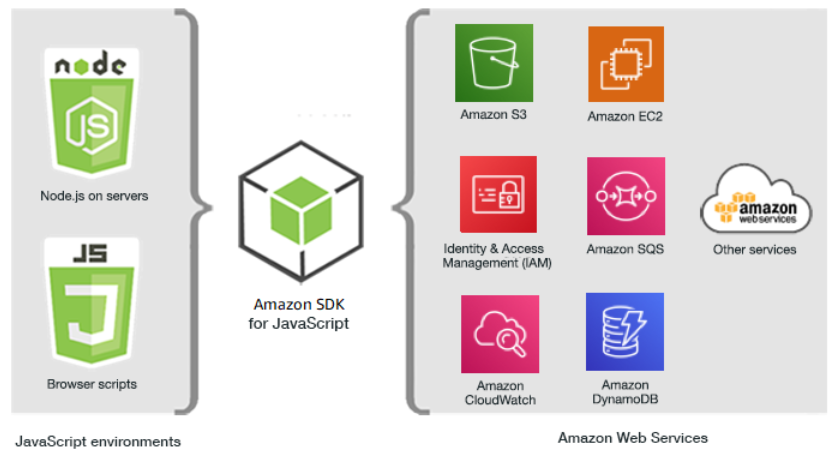
\includegraphics[width=0.9\textwidth]{images/AWSSDK.png}  % Sostituisci 'nome_immagine' con il nome del tuo file immagine e l'estensione
        \caption{The high level rappresentation of the AWS SDK for JavaScript v3 \cite{AWSSDK}}
        \label{fig:AWSSDK}
    \end{figure}
    \item AWS CDK: The AWS Cloud Development Kit (CDK) "is an open-source software development framework for defining cloud infrastructure in code and provisioning it through AWS CloudFormation" \cite{WhatIsTheAWSCDK}. This tool was used in the final phase of the POC design to automate the creation of the stack comprising all the services used.
    \item AWS IoT Core: AWS IoT Core provides the ability to connect IoT devices to AWS cloud services. AWS IoT Core enables the connection of IoT devices to AWS cloud services. It simplifies the integration of IoT devices with other AWS services. This is especially relevant in the automotive industry, where vehicle system ECUs can be viewed as multiple IoT devices. Communication between the device and AWS services can occur in several modes, with the MQTT protocol being the most important for this project. The device can be connected by developing applications that utilize the SDK libraries. Once the data is transmitted, it can be utilized for various purposes such as testing, validation, and analysis.
    \begin{figure}[h]  % 'h' significa che la figura viene posizionata qui
        \centering
        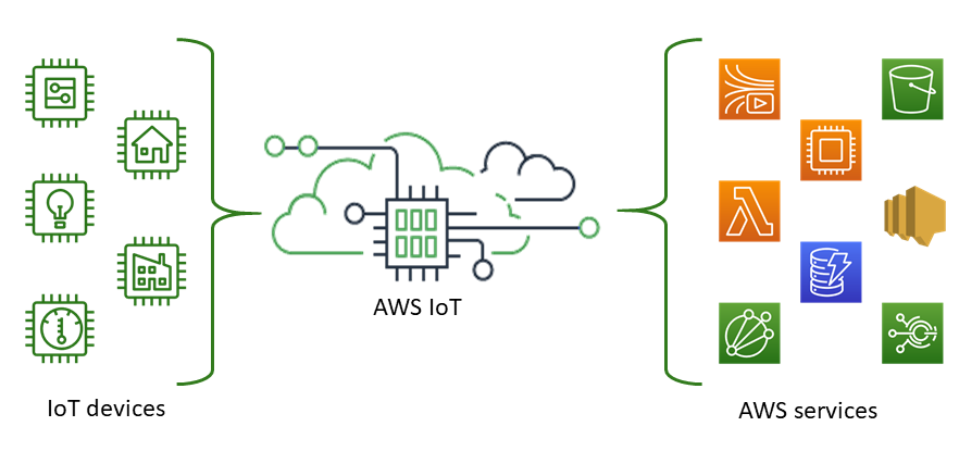
\includegraphics[width=0.9\textwidth]{images/AWSIoTCore.png}  % Sostituisci 'nome_immagine' con il nome del tuo file immagine e l'estensione
        \caption{AWS IoT Core connection system beetween IoT device and AWS service \cite{AWSIoTCore}}
        \label{fig:AWSIoTCore}
    \end{figure}
    \item AWS IoT Greengrass: "AWS IoT Greengrass is an open source Internet of Things (IoT) edge runtime and cloud service that helps you build, deploy and manage IoT applications on devices" \cite{AWSIoTGreengrass}. It is designed to work with intermittent connections and can manage fleets of devices in the field, locally or remotely, using MQTT or other protocols. Once installed, this service can be accessed through the command line. It was utilized in the early stages of project development as an agent to handle updates on the vehicle simulator side. However, this solution will be replaced by a custom solution as explained later.
    \item 
\end{itemize}

\section{Design}
\subsection{Architecture}

\section{Implementation}
\subsection{Code}
\subsection{Tools}

\section{Test and Validation}
\subsection{RPi demo}